\section{Introduction}

Data visualisation is essential to data science and science communication, but
is open to both misinterpretation and misuse: patterns in raw data can be
obscured, statistical assumptions hidden, and effect sizes misrepresented
\cite{weissgerber15}. These concerns can be addressed in part through improved
statistical practices and better plot and chart designs \cite{allen19}, but also
by making visualisations themselves more open and explorable
\cite{dragicevic19}.

Understanding a visualisation requires grasping how it relates to the underlying
data and other visualisations. For example, geoscientists often work with
multiple layered views. To show how these are related, spatial analytics
applications like GeoDa \cite{anselin06} can automatically select the relevant
part of one view as the user changes the selection in a related view, say a
choropleth map. However, this feature is available only if it was specifically
anticipated by the application or library developer; if the geoscientist uses
custom libraries or wants other views linked that the developer did not
consider, they are out of luck.

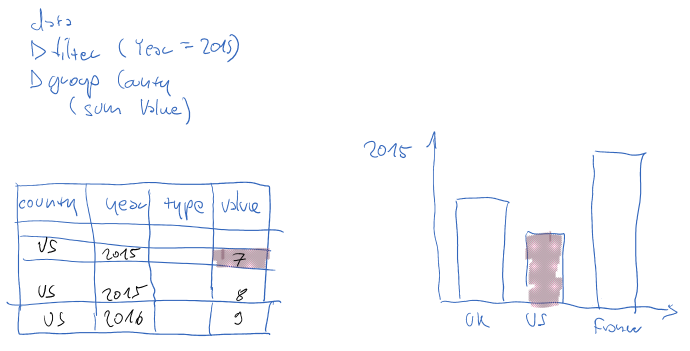
\includegraphics[scale=0.35]{image/chart-fwd}

In this paper we present a framework for authoring visualisations where support
for linking, between data, code, and visualisations is built in, making this
powerful comprehension feature automatic.

\section{Another section}

Our framework provides infrastructure for ``linking'', or multiple-coordinated
views \cite{tobiasz09}, in an application-independent way. The theoretical
foundation of the work is our own prior work on dynamic dependency analysis and
provenance \cite{perera16d, ricciotti17}; in contrast to prior work on
provenance in data visualisation \cite{callahan06}, our approach is much more
fine-grained and is able to associate specific parts of the data or code with
parts of a visualisation in a precise way. While the theoretical technique is
proven, this approach has never been applied to data visualisation before.

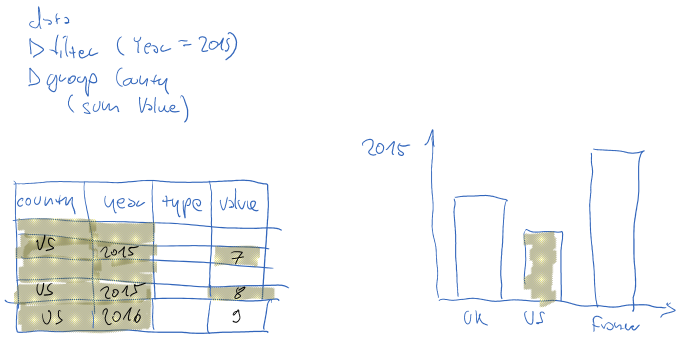
\includegraphics[scale=0.35]{image/chart-bwd}

\section{Conclusions and future work}

There are a number of challenges associated with making our approach practical
and appealing to actual data scientists. A central usability challenge is
visualising these complex relationships between the various parts of a
visualisation and the relevant data and/or visualisation code. This is
essentially a higher-order visualisation problem: visualising information about
the provenance of visualisations. Ideas from temporal data visualisation
\cite{bach16}, data-driven storytelling \cite{bach18}, and ``literate''
visualisation \cite{wood19} may inform our efforts here.
